\subsection{Application example}
We implement the solution proposed by the Manieri et al. in a dedicated algorithm, which is tested in the aforementioned use case of the PEV recharge problem. The challenge involves determining the best charging schedule for a fleet of $m$ vehicles that need to be charged overnight to achieve a specified battery state of charge by the following morning. This plan is organized over a period broken down into $N$ time slots of duration $T$, corresponding to the prediction horizon of a MPC controller. 
\\The upcoming discussion is mainly based on the scenario described in Liberati et al. (2023)\supercite{liberati}.

\subsubsection{Problem definition}
The goal is to compute the optimal charging/discharging schedule for a set of $m$ PEVs connected to the power grid.

Let $P = \begin{bmatrix}
    P_1^T & \dots & P_m^T
\end{bmatrix}^T$, with $P_{p} \in \mathbb{R}^N$ being the difference between the charging and discharging power schedules of PEV $p = 1, \dots, m$ over the prediction horizon of duration $N$, given by:
\begin{align}
    P_{p} \doteq P^{ch}_{p}-P^{dis}_{p}, \quad \forall p. \label{constr:c1}
\end{align}
At each time slot $t = 1, \dots, N$, each PEV can be exclusively charged or discharged within eligibility intervals:
\begin{gather}
    \delta^{ch}_{p} P^{ch,min}_p \leq P^{ch}_{p} \leq \delta^{ch}_{p} P^{ch,max}_p, \quad \forall p, \label{constr:c2}\\
    \delta^{dis}_{p} P^{dis,min}_p \leq P^{dis}_{p} \leq \delta^{dis}_{p} P^{dis,max}_p, \quad \forall p, \label{constr:c3}\\
    \delta^{dis}_{p} + \delta^{ch}_{p} \leq 1, \quad \forall p. \label{constr:c4}
\end{gather}
Here, \ref{constr:c4} guarantees the mutual exclusiveness of the charging/discharging processes, since $\delta^{ch}_{p}, \delta^{dis}_{p} \in \{0,1\}$ are boolean variables that determine the charging and discharging status of PEV $p$ at time $t$. Meanwhile, \ref{constr:c2} and \ref{constr:c3} ensure that the power injected into or drawn from the battery is within the limits.

The aggregated power profile of the fleet is simply the sum of the individual PEV power profiles, and it has to comply with the maximum power limit constraint $P^{max}$ imposed by the distribution system operator:
\begin{gather}
    P^{agg} \doteq \sum_{p=1}^m P_{p}, \label{constr:c5}\\
    P^{agg} \leq P^{max}. \label{constr:c6}
\end{gather}

The state of charge of PEV $p$, namely $x_p$, evolves in time according to the following equation:
\begin{align}
    \begin{cases}
        x_{p}(t+1) = x_{p}(t) + T (\eta^{ch}_p P^{ch}_{p} - \frac{1}{\eta^{dis}_p} P^{dis}_{p}) \label{constr:c7}\\
        x_{p}(t_0) = (x_0)_p
    \end{cases}
    \quad \forall p,
\end{align}
where $t_0$ is the initial time slot, $(x_0)_p$ is the initial state of charge, and $\eta^{ch}_p$ and $\eta^{dis}_p$ are the charging and discharging efficiencies.\\
Some of the local constraints arise from the preferences of the PEV owners, who have the faculty to express the desired duration and final level of charge of the process; some other, instead, depend on the physical limitations of the battery, such as the minimum and maximum state of charge $x^{min}_p$ and $x^{max}_p$:
\begin{gather}
    x_{p}(F_p) = x^{ref}_p, \quad \forall p, \label{constr:c8}\\
    x^{min}_p \leq x_{p} \leq x^{max}_p, \quad \forall p. \label{constr:c9}
\end{gather}

Finally, the objective function to minimize is the following:
\begin{align}
    V \doteq \sum_{p=1}^m \xi_{p}^T P_{p} \label{cost},
\end{align}
where small perturbation array $\xi_{p}$ is introduced, weighting the power to satisfy Assumption 2.4 of Vujanic et al. (2014)\supercite{vujanic}.

\subsubsection{Solution algorithms}
In this subsection, we implement the algorithms proposed in Manieri et al. (2023)\supercite{manieri} by adapting them to the problem at hand.

Given a value of the tightening array $\rho$, Algorithm \ref{alg:2} is able to compute the corresponding solution couple $[P^{LP}_{\rho}, P(\lambda^*_{\rho})]$. $P^{LP}_{\rho}$ is the solution of the linear program corresponding to the restricted\footnotemark[1] version of the convexified problem \ref{eq:LP}, while $\lambda^*_{\rho}$ is the solution to the restricted\footnotemark[1] version of the dual problem \ref{eq:dual}. In particular, the Lagrange multiplier $\lambda$ is updated through \ref{eq:lambda} with the solution of \ref{eq:inner} found using the last available value of $\lambda$ until convergence. Once $\lambda$ is at convergence, the code constructs the sequence $\hat{P}(h)$, whose accumulation points are shown to be solutions of the restricted\footnotemark[1] version of \ref{eq:LP}\footnote[2]{One can prove that $\lim{h \to \infty} \hat{P}(h) = P^{LP}_\rho$.}. When $\hat{P}(h)$ is also at convergence, its most recent value is selected as the estimate of $P_\rho^{LP}$. On the other hand, once lambda has converged, each solution found in steps $4$-$6$ is a valid $P(\lambda^*_{\rho})$; among these, only the cheapest one is selected (steps $14$-$16$).

Algorithm \ref{alg:1} allows to compute the optimal power schedule $P^*$ for the PEVs. After initializing the resource restriction array $\rho$ at zero, iteratively Algorithm \ref{alg:2} is employed in order to find $[P^{LP}_{\rho(k)}, P(\lambda^*_{\rho(k)})]$, and if the latter is feasible and it is better than any previous one in terms of cost, it is stored, together with its cost, as the current optimal solution. Finally, the tightening array $\rho$ is updated according to \ref{eq:rho_update}, and the process is repeated until a stopping condition is met.

\begin{algorithm}[H]
    \caption{Computation of $P^*$.}
    \label{alg:1}

    \setstretch{1.2}
    \KwOut{$P^*$}
    $\rho(0) = 0$\;
    $V^* = \infty$\;
    
    \For{$k = 0, 1, 2, \dots$}{
        $[P^{LP}_{\rho(k)}, P(\lambda^*_{\rho(k)})] = $ \textbf{Algorithm 2}($\rho(k)$)\;
        $P^{agg}(k) = \sum_{p=1}^m P_p(\lambda^*_{\rho(k)})$\;
        $V(k) = \sum_{p=1}^m \xi_{p}^T P_p(\lambda^*_{\rho(k)})$\;
        \If{$P^{agg}(k) \leq P^{max} \land V(k) \leq V^*$}
        {
            $P^* = P(\lambda^*_{\rho(k)})$\;
            $V^* = V(k)$\;
        }
        $\rho(k+1) = \left[ \sum_{p = 1}^m P_p(\lambda^*_{\rho(k)}) - P^{LP}_{p, \rho(k)} \right]_+$\;
    }
    \Return $P^*$\;
\end{algorithm}

\begin{algorithm}[H]
    \caption{Computation of [$P^{LP}_{\rho}$, $P(\lambda^*_{\rho})$].}
    \label{alg:2}

    \setstretch{1.2}
    \KwIn{$\rho$}
    \KwOut{$P^{LP}_{\rho(k)}$, $P(\lambda^*_{\rho(k)})$}
    
    $\lambda(0) = 0$\;
    $h = 1$\;
    
    \For{$l = 1, 2, \dots$}{
        \For{$p = 1, \dots, m$}{
            $P_p(l) = \arg \min_{P_p} \left\{ \left(\xi_p^T + \lambda^T(l)\right) P_p \right\}$ \\ \hfill s.t. \ref{constr:c1}-\ref{constr:c4}, \ref{constr:c7}-\ref{constr:c9}\;
        }
        $\gamma(l) = \sum_{p=1}^m P_p(l) -P^{max} + \rho $\;
        $\lambda(l+1) = \left[ \lambda(l) + \alpha(l) \gamma(l) \right]_+$\;
        \If{$\lambda$ is at convergence}
        {
            \For{p = 1, \dots, m}{
                $\hat{P}_p(h) = \frac{\sum_{\tau = l-h}^l \alpha(\tau) P_p(\tau)}{\sum_{\tau= l-h}^l \alpha(\tau)}$\; 
            }
            \If{$\hat{P}(h)$ is at convergence}{
                $P^{LP}_{\rho} = \hat{P}(h)$\;
                \For{$p=1, \dots, m$}{
                    $P_p(\lambda^*_{\rho}) = \arg \min_{P_p} \xi_p^T P_p$ \\ \hfill s.t. $ P_p = P_p(\tau): \tau \geq l-h$\;
                }
                \Return $P^{LP}_{\rho}$, $P(\lambda^*_{\rho})$\;
            }
            $h + +$\;
        }
    }
\end{algorithm}

\subsubsection{Numerical results}
First of all, it is necessary to recall the results of the numerical simulations carried out in Manieri et al. (2023)\supercite{manieri}. The authors, in fact, report having observed not only that the optimality gap between the solutions of \ref{eq:MILP} and \ref{eq:BAR} tends to zero as the number of agents $m$ increases according to \ref{eq:ratio} just as aforementioned for the cases of Vujanic et al. (2014)\supercite{vujanic} and Falsone et al. (2019)\supercite{falsone}, but that in this case it even sits some orders of magnitude below. This outstanding improvement clearly derives from a decrease in the level of conservativity of the approach, which however occurs at the cost of increased difficulty in identifying an admissible solution (as already mentioned, in fact, the guarantee of finding it persists only when $\beta=1$).

Our simulations were performed adopting the parameters in Table \ref{tab:sim_param} using \textit{MATLAB R2024a}. The \textit{Optimization Toolbox} and the \textit{Global Optimization Toolbox} provided the utilities to solve the MILP problems (in particular, the \textit{intlinprog} solver), while \textit{Parallel Computing Toolbox} was exploited to take avantage of the modularity of the decentralized problem in order to speed up the computation employing multiple CPU cores, each effectively corrisponding to a cluster of PEVs.

\begin{table}[H]
    \centering
    \begin{tabular}{|c|c|}
        \hline
        Symbol & Value \\
        \hline
        $m$ & $500$ \\
        $N = F_p$ & $24$ \\
        $T$ [min] & $20$ \\
        $P^{max}$ [kW] & $\{400, 200, 600\}$ \\
        $P^{max}_p$ [kW] & $3.3$ \\
        $x^{max}_p$ [kWh] & $[8, 16]$ \\
        $x^{min}_p$ [kWh] & $1$ \\
        $(x_0)_p$ [kWh] & $[0.2, 0.5] \cdot x^{max}_p$ \\
        $x_p(F_p)$ [kWh] & $[0.55, 0.8] \cdot x^{max}_p$ \\
        $\eta^{ch}_p$ & $[0.925, 0.985]$ \\
        $\xi_p$ & $[0, 0.3]$ \\
        \hline
    \end{tabular}
    \caption{Simulation parameters.}
    \label{tab:sim_param}
\end{table}

\noindent The simulations were carried out setting the step-size $\alpha$ in Algorithm \ref{alg:2} to $\frac{0.01}{n+1}$. Moreover, since as just mentioned the procedure does not guarantee the feasibility of the solution, we introduced a tolerance of $5\%$ on the aggregated power constraint violation, meaning that all solutions with a violation below this threshold were considered feasible.\\
Iteratively (and up to iteration $25$, where we stopped), the percentage of violation of the coupling constraint descended under the set threshold, as shown in Figure \ref{fig:violation}, due to the evolution of the resource restriction array $\rho$ (whose norm is plotted in Fig. \ref{fig:norm_rho}). 

\begin{figure}[H]
    \centering
    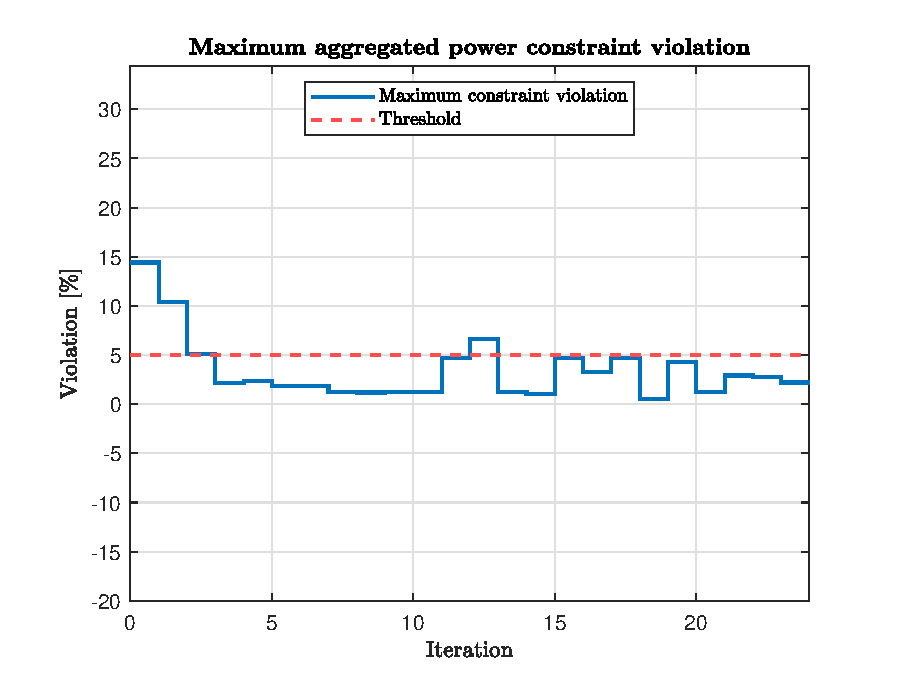
\includegraphics[width=0.9\columnwidth]{assets/violation.eps}
    \caption{Maximum percentage aggregated power constraint violation per iteration. }
    \label{fig:violation}
\end{figure}

\begin{figure}[H]
    \centering
    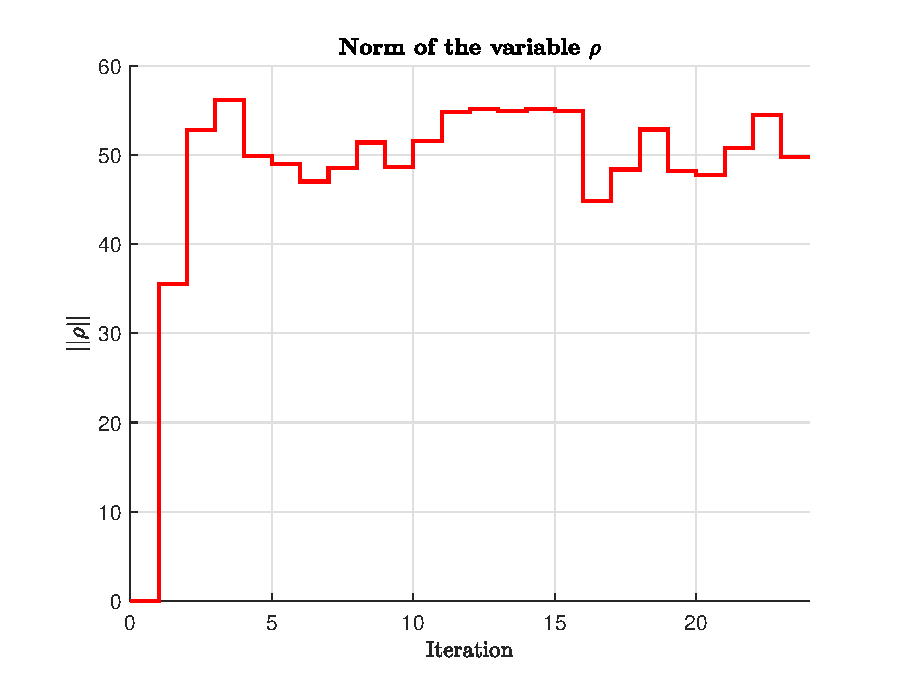
\includegraphics[width=0.9\columnwidth]{assets/norm_rho.eps}
    \caption{Norm of the resource restriction array per iteration. }
    \label{fig:norm_rho}
\end{figure}

\begin{figure}[H]
    \centering
    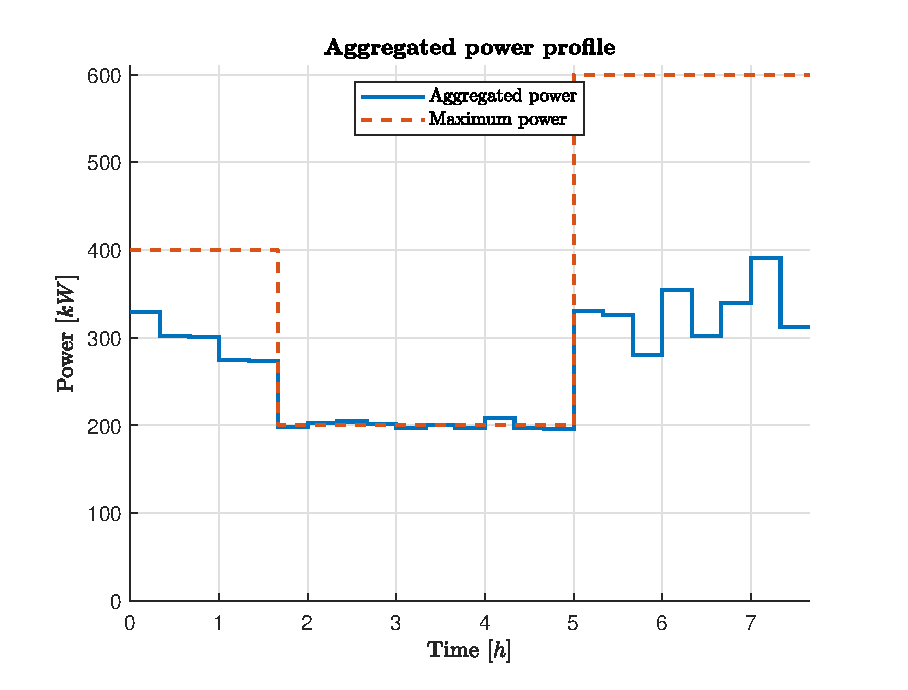
\includegraphics[width=0.9\columnwidth]{assets/aggregated.eps}
    \caption{Maximum and actual aggregated power profiles. }
    \label{fig:aggregated}
\end{figure}

\noindent The lowest-cost solution found among those examined is depicted in Fig. \ref{fig:aggregated}, together with the maximum aggregated power profile to be satisfied. In Fig. \ref{fig:soc}, the state of charge of a random batch of $10$ PEVs is shown, highlighting the convergence to the desired final level of charge.

\begin{figure}[H]
    \centering
    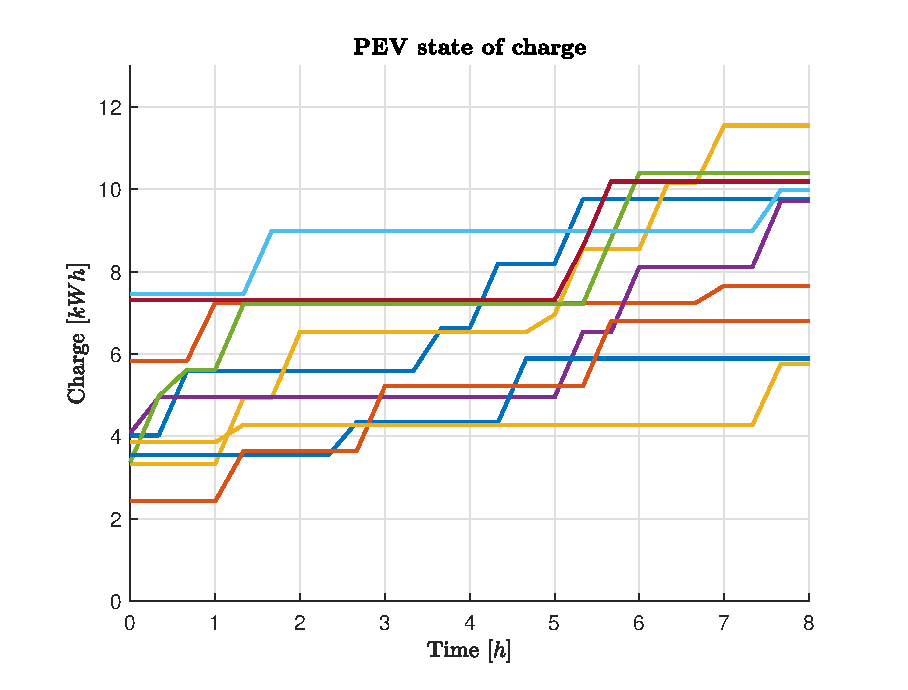
\includegraphics[width=0.9\columnwidth]{assets/state_of_charge.eps}
    \caption{State of charge of 10 random PEVs. }
    \label{fig:soc}
\end{figure}

Being computed in a decentralized way, as one would expect the solution at issue was found taking a much shorter amount of time than the MPC sampling time, namely about $19.4$ seconds\footnote[3]{Mind that this duration is estimated and not directly measured, as that the number of cores of the computer CPU is less than $m$.} ($<< 20$ minutes). However, this duration is considerably longer than that of the other procedures (for comparison, see Liberati et al (2023)\supercite{liberati}, where, despite the presence of a greater number of constraints due to the reference tracking objective, the computation time is approximately $1$ second).

Finally, we further tested the procedure by varying the quantity of PEVs of which the fleet is made up (of course, the maximum aggregated power constraint varied accordingly). The results obtained show that the maximum violation of the coupling constraint is greater the smaller the number of agents involved, and they are directly linked to what both the authors and the theory suggest in terms of optimality gap (related to, once again, \ref{eq:ratio}).

\begin{table}[H]
    \centering
    \begin{tabular}{|c|c|}
        \hline
        $m$ & Violation \\
        \hline
        20  & 40.97 \% \\
        50  & 14.66 \% \\
        100 & 10.26 \% \\
        200 & 8.65 \% \\
        500 & 3.46 \% \\
        \hline
    \end{tabular}
    \label{table:violation}
    \caption{Mean global constraint violation on 25 runs for different numbers of PEVs.}
\end{table}